% ------------------------------------------------------------------------------
% TYPO3 CMS 6.2 LTS - What's New - Chapter "Backend Changes" (German Version)
%
% @author	Michael Schams <schams.net>
% @license	Creative Commons BY-NC-SA 3.0
% @link		http://typo3.org/download/release-notes/whats-new/
% @language	German
% ------------------------------------------------------------------------------
% Chapter: Backend Changes
% ------------------------------------------------------------------------------

\section{Änderungen im Backend}
\begin{frame}[fragile]
	\frametitle{Änderungen im Backend}

	\begin{center}\huge{Kapitel 3:}\end{center}
	\begin{center}\huge{\color{typo3darkgrey}\textbf{Änderungen im Backend}}\end{center}

\end{frame}

% ------------------------------------------------------------------------------
% Autofocus
% ------------------------------------------------------------------------------
% http://forge.typo3.org/issues/49228

\begin{frame}[fragile]
	\frametitle{Änderungen im Backend}
	\framesubtitle{Anmeldung am Backend}

 	\begin{itemize}
		\item Autofokus auf das Eingabefeld des Benutzernamens bei Aufruf des Anmeldeformulars\newline
			\small(HTML5 Attribute: \texttt{autofocus="autofocus"})\normalsize
	\end{itemize}

	\begin{figure}
		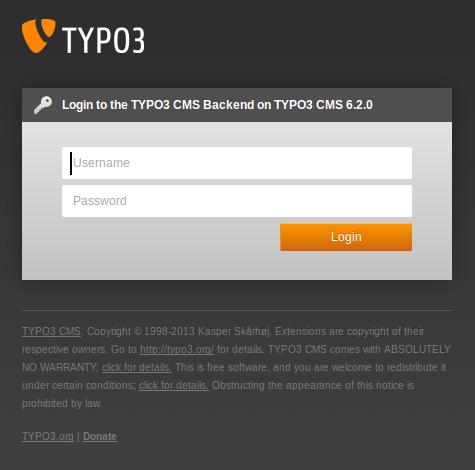
\includegraphics[width=0.35\linewidth]{Images/BackendChanges/BackendLogin.png}
	\end{figure}

\end{frame}

% ------------------------------------------------------------------------------
% Visual Appearance
% ------------------------------------------------------------------------------
% http://forge.typo3.org/issues/48376

\begin{frame}[fragile]
	\frametitle{Änderungen im Backend}
	\framesubtitle{Allgemeines Erscheinungsbild}

	\begin{columns}[T]

		\begin{column}{.5\textwidth}
			\begin{itemize}
				\item Verbesserte Usability durch aufgelockertes Erscheinungsbild
				\item Horizontale und vertikale Abstände vieler Elemente wurden vergrößert
				\item Basis ist ein 12 Pixel Raster, welches verdoppelt wurde
			\end{itemize}

			\advance\leftskip+3.6cm

			\smaller
				Links: TYPO3 4.5\newline
				Rechts: TYPO3 6.2
			\normalsize
		\end{column}

		\begin{column}{.5\textwidth}
			\begin{figure}\vspace*{-0.4cm}
				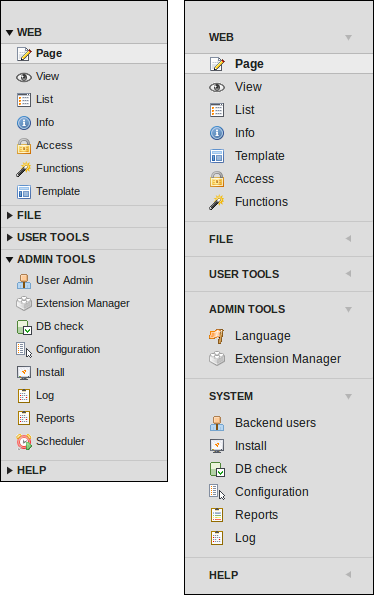
\includegraphics[width=0.6\linewidth]{Images/BackendChanges/VisualAppearance.png}
			\end{figure}
		\end{column}

	\end{columns}

\end{frame}

% ------------------------------------------------------------------------------
% Visual Appearance
% ------------------------------------------------------------------------------

\begin{frame}[fragile]
	\frametitle{Änderungen im Backend}
	\framesubtitle{Allgemeines Erscheinungsbild}

	\begin{columns}[T]

		\begin{column}{.5\textwidth}

			\begin{itemize}
				\item Modul in der linken Spalte wurden neu angeordnet
				\item Modul "ADMINWERKZEUGE" wurde zweigeteilt:

					\begin{itemize}
						\item \textbf{ADMINWERKZEUGE} ("Sprache" und "Erweiterungsmanager")
						\item \textbf{SYSTEM} (low-level Tools, die keinen Seitenbaum anzeigen)
					\end{itemize}

				\item Das Modul "TypoScript-Hilfe" wurde entfernt (veraltet)

			\end{itemize}

		\end{column}

		\begin{column}{.5\textwidth}
			\begin{figure}\vspace*{-0.4cm}
				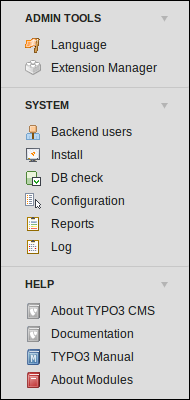
\includegraphics[width=0.35\linewidth]{Images/BackendChanges/AdminTools.png}
			\end{figure}
		\end{column}

	\end{columns}

\end{frame}

% ------------------------------------------------------------------------------
% Visual Appearance
% ------------------------------------------------------------------------------
% http://forge.typo3.org/issues/36017

\begin{frame}[fragile]
	\frametitle{Änderungen im Backend}
	\framesubtitle{Allgemeines Erscheinungsbild}

	\begin{itemize}
		\item \texttt{<h1>}-Überschriften im rechten Bereich werden nun durchgehend im TYPO3 Font dargestellt
	\end{itemize}

	\begin{figure}
		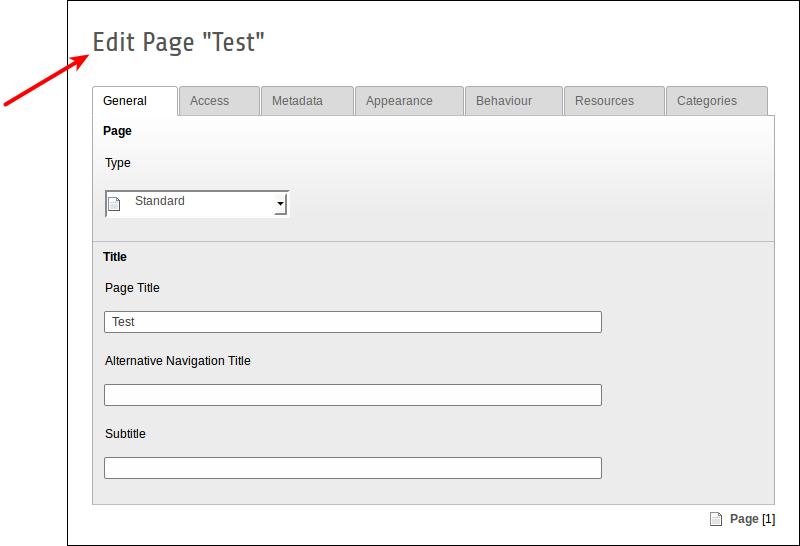
\includegraphics[width=0.6\linewidth]{Images/BackendChanges/ConsistantFont.png}
	\end{figure}

\end{frame}

% ------------------------------------------------------------------------------
% Visual Appearance
% ------------------------------------------------------------------------------
% http://forge.typo3.org/issues/41631

\begin{frame}[fragile]
	\frametitle{Änderungen im Backend}
	\framesubtitle{Allgemeines Erscheinungsbild}

	\begin{itemize}
		\item Modul "Reports" hat ein eigenes Symbol erhalten
	\end{itemize}

	\begin{figure}
		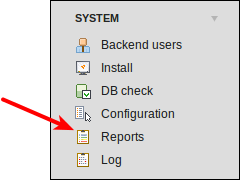
\includegraphics[width=0.35\linewidth]{Images/BackendChanges/ModuleReportsIcon.png}
	\end{figure}

\end{frame}

% ------------------------------------------------------------------------------
% Filelist: Drag&Drop File Upload
% ------------------------------------------------------------------------------
% http://forge.typo3.org/issues/47005

\begin{frame}[fragile]
	\frametitle{Änderungen im Backend}
	\framesubtitle{Drag\&Drop in der Dateiliste}

	\begin{itemize}
		\item In der Dateiliste können nun Dateien per HTML5 Drag\&Drop hochgeladen werden
	\end{itemize}

	\begin{figure}
		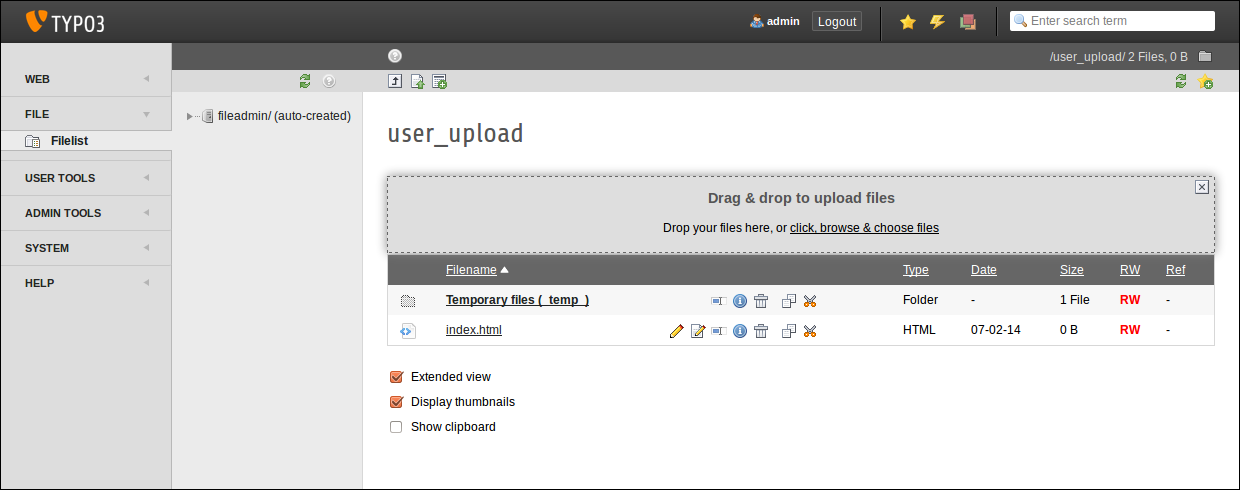
\includegraphics[width=0.95\linewidth]{Images/BackendChanges/DragDropFileUpload.png}
	\end{figure}

\end{frame}

% ------------------------------------------------------------------------------
% Filelist: Drag&Drop File Upload
% ------------------------------------------------------------------------------
% http://forge.typo3.org/issues/47005

\begin{frame}[fragile]
	\frametitle{Änderungen im Backend}
	\framesubtitle{Drag\&Drop in der Dateiliste}

	\begin{itemize}
		\item ...sowie über Inhaltselemente (Button: "Select \& upload files")

	\end{itemize}

	\begin{figure}
		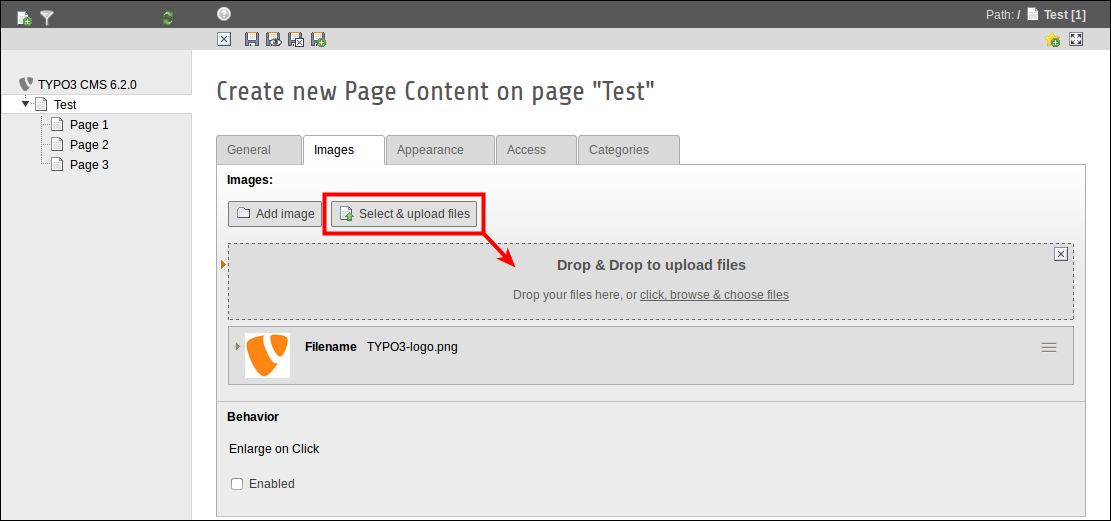
\includegraphics[width=0.95\linewidth]{Images/BackendChanges/SelectAndUploadFiles.png}
	\end{figure}

\end{frame}

% ------------------------------------------------------------------------------
% Backend Users
% ------------------------------------------------------------------------------
% http://forge.typo3.org/issues/43053

\begin{frame}[fragile]
	\frametitle{Änderungen im Backend}
	\framesubtitle{Backend Benutzerverwaltung}

	\begin{itemize}
		\item Neben dem Benutzernamen wird nun auch der Realname dargestellt
		\item Klick auf den Namen führt zum Bearbeitungsformular
		\item Zudem gibt es nun einen Delete-Button in der Liste
	\end{itemize}

	\begin{figure}
		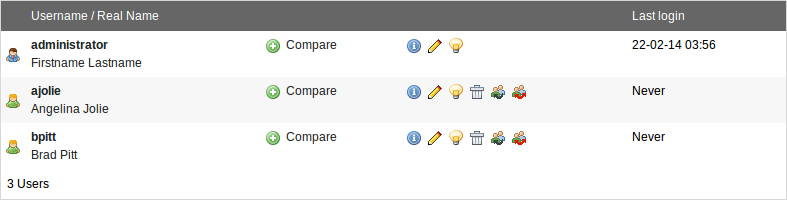
\includegraphics[width=0.95\linewidth]{Images/BackendChanges/BackendUserList.png}
	\end{figure}

\end{frame}

% ------------------------------------------------------------------------------
% Live Search
% ------------------------------------------------------------------------------
% http://forge.typo3.org/issues/35358

\begin{frame}[fragile]
	\frametitle{Änderungen im Backend}
	\framesubtitle{Verbesserte Suchfunktion}

	\begin{itemize}
		\item Die Live-Suche zeigt nun UID und PID als Tooltip in der Ergebnisliste an
		\item Sobald man nach einer Suche das Editierformular wieder schließt, gelangt man in die Listen-Ansicht der PID (und nicht wie früher auf eine leere Seite)
	\end{itemize}

	\begin{figure}
		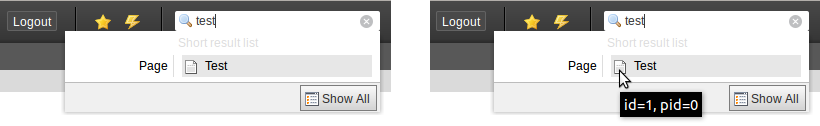
\includegraphics[width=0.8\linewidth]{Images/BackendChanges/LiveSearchTooltip.png}
	\end{figure}

\end{frame}

% ------------------------------------------------------------------------------
% Live Search
% ------------------------------------------------------------------------------

\begin{frame}[fragile]
	\frametitle{Änderungen im Backend}
	\framesubtitle{Live Search}

	\begin{itemize}
		\item In TYPO3 vor Version 6.2 durchsucht die Live-Suche für Seiten nur die Felder \texttt{title} und \texttt{uid}
		\item Ab TYPO3 Version 6.2 kann nun das Feld \texttt{alias} zusätzlich in der Suche einbezogen werden, sofern per UserTSconfig konfiguriert\newline
			\smaller(\texttt{options.pageTree.searchInAlias = 1})\normalsize
	\end{itemize}

	\begin{figure}
		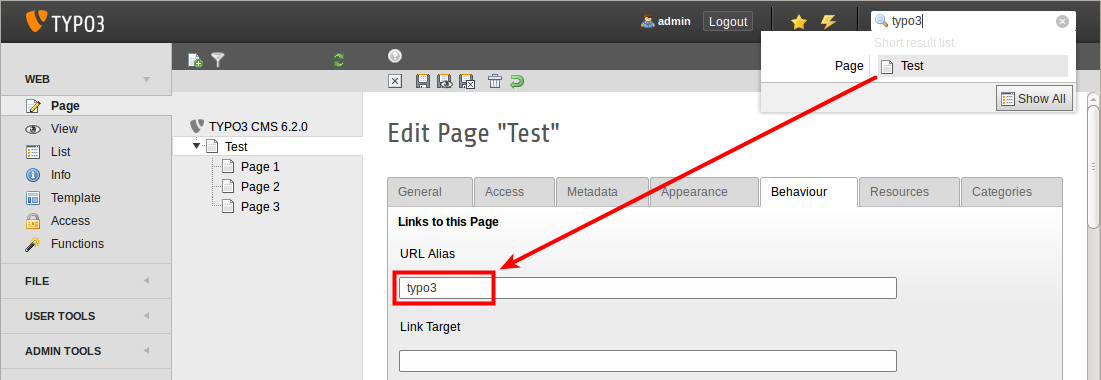
\includegraphics[width=0.8\linewidth]{Images/BackendChanges/LiveSearchInAlias.png}
	\end{figure}

\end{frame}

% ------------------------------------------------------------------------------
% File Abstraction Layer
% ------------------------------------------------------------------------------

\begin{frame}[fragile]
	\frametitle{Änderungen im Backend}
	\framesubtitle{File Abstraction Layer}

	\begin{itemize}
		\item Dateiname und Titel werden nun im FAL-Element "Header" angegeben
	\end{itemize}

	\begin{figure}
		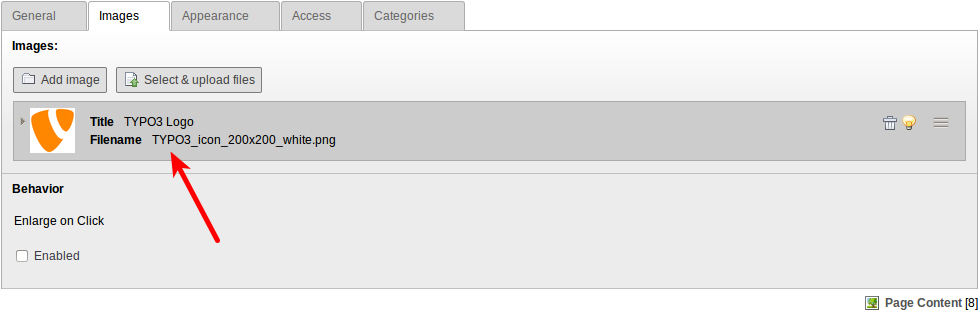
\includegraphics[width=0.95\linewidth]{Images/BackendChanges/FalTitleAndFilename.png}
	\end{figure}

\end{frame}

% ------------------------------------------------------------------------------
% File Abstraction Layer
% ------------------------------------------------------------------------------

\begin{frame}[fragile]
	\frametitle{Änderungen im Backend}
	\framesubtitle{File Abstraction Layer (EXT:filemetadata)}

	\begin{itemize}
		\item Durch die EXT:filemetadata werden zusätzliche Metadaten eingebracht\newline
			\smaller(Extension wird mitgeliefert, ist aber standardmäßig nicht installiert)\normalsize
	\end{itemize}

	\begin{figure}
		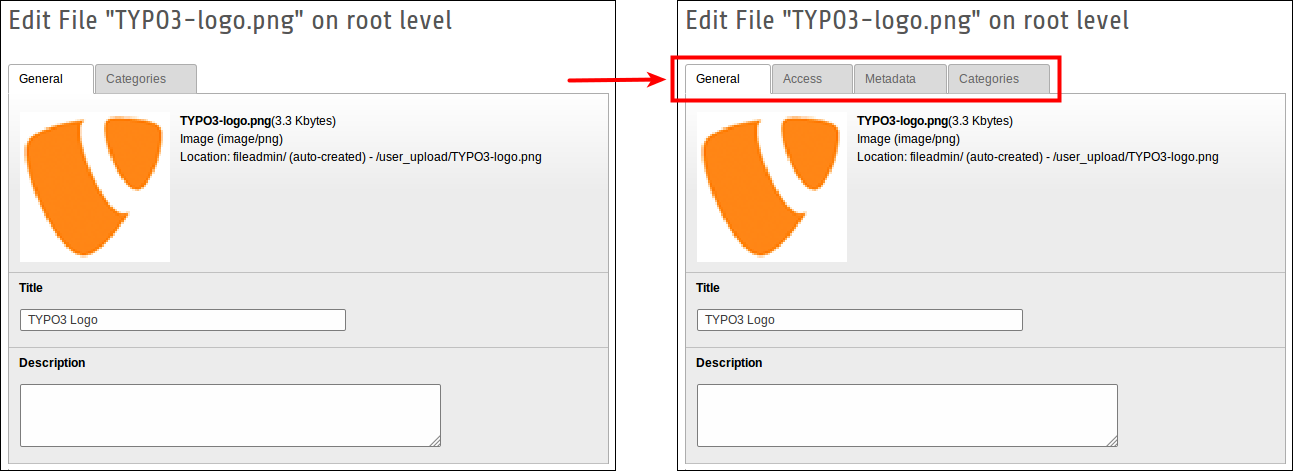
\includegraphics[width=0.95\linewidth]{Images/BackendChanges/FileMetaDataTabs.png}
	\end{figure}

\end{frame}

% ------------------------------------------------------------------------------
% File Abstraction Layer
% ------------------------------------------------------------------------------

\begin{frame}[fragile]
	\frametitle{Backend Changes}
	\framesubtitle{File Abstraction Layer (EXT:filemetadata)}

	\begin{figure}
		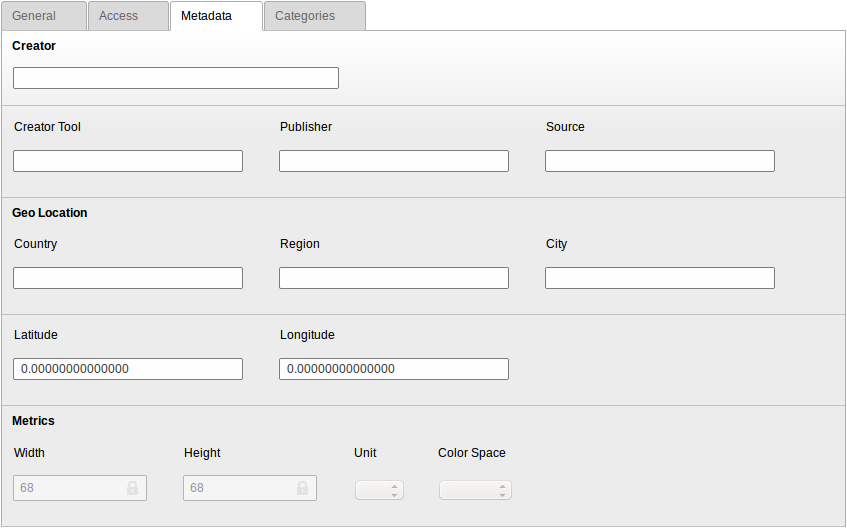
\includegraphics[width=0.8\linewidth]{Images/BackendChanges/FileMetaData.png}
	\end{figure}

\end{frame}

% ------------------------------------------------------------------------------
% File Abstraction Layer
% ------------------------------------------------------------------------------

\begin{frame}[fragile]
	\frametitle{Änderungen im Backend}
	\framesubtitle{File Abstraction Layer}

	\begin{itemize}
		\item FAL Metadaten können nun in Frontend-Sprachen übersetzt werden
	\end{itemize}

	\begin{figure}
		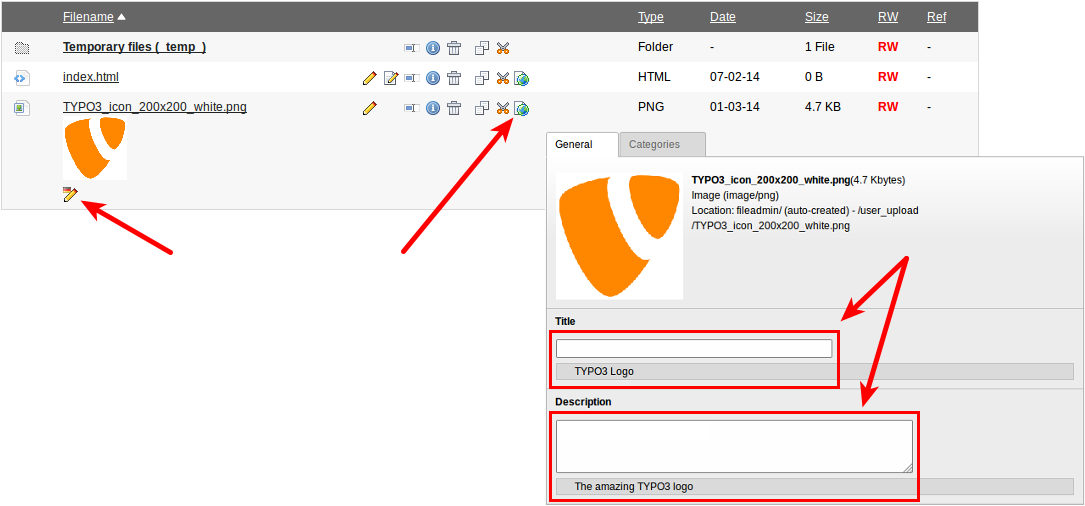
\includegraphics[width=0.95\linewidth]{Images/BackendChanges/FalTranslateMetaData.png}
	\end{figure}

\end{frame}

% ------------------------------------------------------------------------------
% Module: Documentation
% ------------------------------------------------------------------------------

\begin{frame}[fragile]
	\frametitle{Änderungen im Backend}
	\framesubtitle{Modul: Documentation}

	\begin{columns}[T]

		\begin{column}{.5\textwidth}
			\begin{itemize}
				\item Neues Modul "Documentation" ermöglicht es, Dokumentationen herunterzuladen
				\item Das Modul wird über den Erweiterungsmanager hinzugefügt, bzw. ist bei neuen Installationen bereits standardmäßig geladen
				\item Funktion "Download Documentation" lädt Dokumentationen nach
			\end{itemize}
		\end{column}

		\begin{column}{.5\textwidth}
			\begin{figure}\vspace*{-0.4cm}
				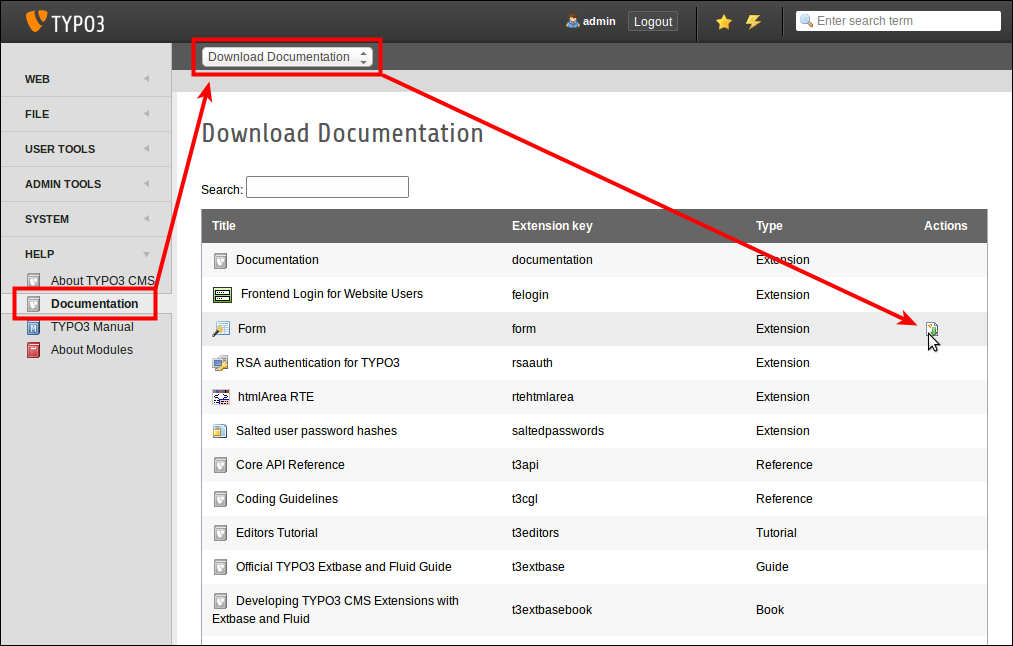
\includegraphics[width=1\linewidth]{Images/BackendChanges/DownloadDocumentation.png}
			\end{figure}
		\end{column}

	\end{columns}

\end{frame}

% ------------------------------------------------------------------------------
% Module: Documentation
% ------------------------------------------------------------------------------

\begin{frame}[fragile]
	\frametitle{Änderungen im Backend}
	\framesubtitle{Modul: Documentation}

	\begin{itemize}
		\item Im Modul "Show Documentation" kann man die Dokumentationen dann ansehen
	\end{itemize}

	\begin{figure}
		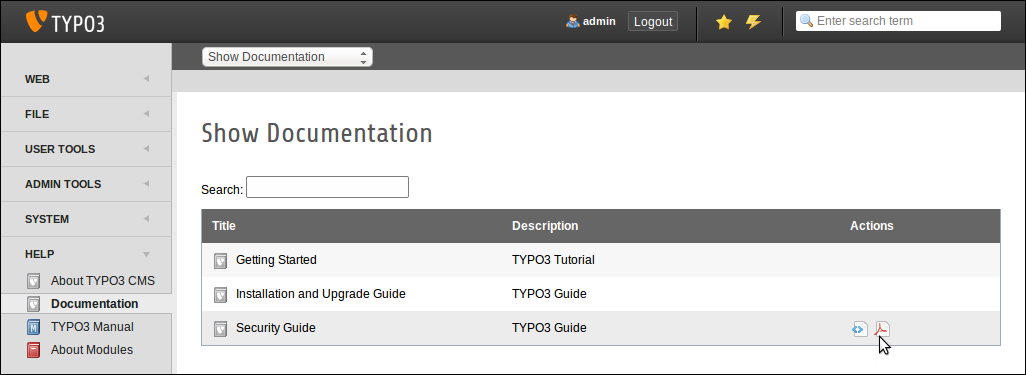
\includegraphics[width=0.95\linewidth]{Images/BackendChanges/ShowDocumentation.png}
	\end{figure}

\end{frame}

% ------------------------------------------------------------------------------
% Removed: TypoScript Help
% ------------------------------------------------------------------------------
% http://forge.typo3.org/issues/47931

\begin{frame}[fragile]
	\frametitle{Änderungen im Backend}
	\framesubtitle{Removed: TypoScript Help}

 	\begin{itemize}
		\item EXT:tsconfig\_help ("TypoScript-Hilfe") entfernt\newline
			\small(enthielt veraltete Information und wurde seit längerem nicht gepflegt)
	\end{itemize}

	\begin{figure}
		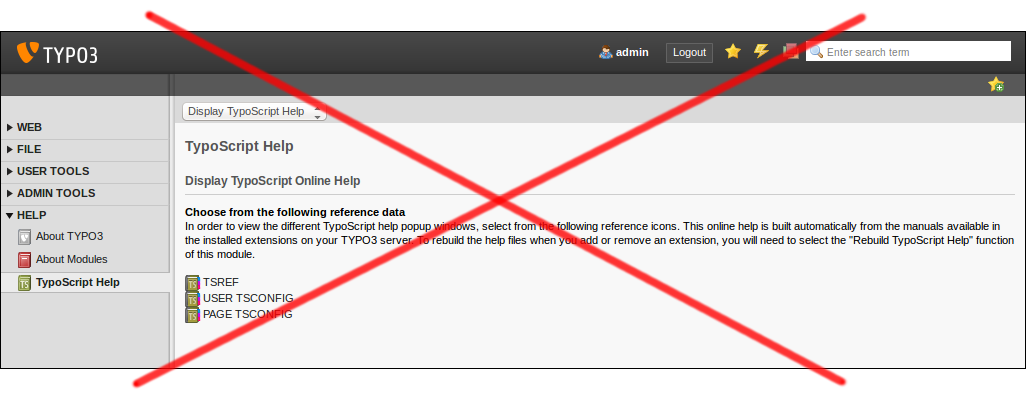
\includegraphics[width=0.95\linewidth]{Images/BackendChanges/TypoScriptHelpRemovedCrossed.png}
	\end{figure}

\end{frame}


% ------------------------------------------------------------------------------
% Scheduler
% ------------------------------------------------------------------------------

\begin{frame}[fragile]
	\frametitle{Änderungen im Backend}
	\framesubtitle{Planer ("Scheduler")}

	\begin{itemize}
		\item Löschen von Scheduler-Tasks in der Bearbeitungsansicht\newline
			\small(in TYPO3 vor Version 6.2 können Tasks nur in der Listenansicht gelöscht werden)\normalsize
	\end{itemize}

	\begin{figure}
		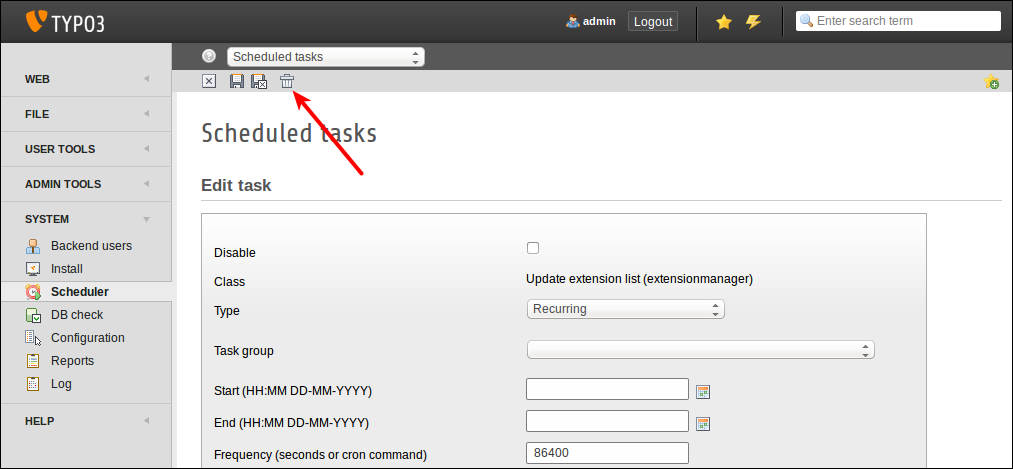
\includegraphics[width=0.95\linewidth]{Images/BackendChanges/DeleteSchedulerTaskInEditView.png}
	\end{figure}

\end{frame}

% ------------------------------------------------------------------------------
% Scheduler
% ------------------------------------------------------------------------------

\begin{frame}[fragile]
	\frametitle{Änderungen im Backend}
	\framesubtitle{Planer ("Scheduler")}

	\begin{itemize}
		\item Scheduler-Tasks können nun mit einer Beschreibung versehen werden\newline
			\small(als Subheadline oder Tooltip, siehe nächste Seite)\normalsize
	\end{itemize}

	\begin{figure}
		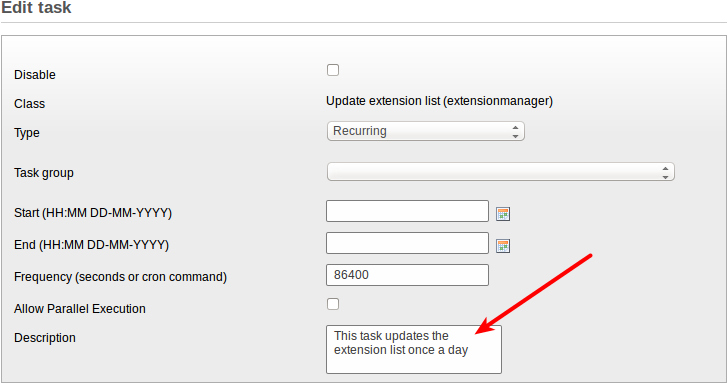
\includegraphics[width=0.7\linewidth]{Images/BackendChanges/SchedulerTaskDescription.png}
	\end{figure}

\end{frame}

% ------------------------------------------------------------------------------
% Scheduler
% ------------------------------------------------------------------------------

\begin{frame}[fragile]
	\frametitle{Änderungen im Backend}
	\framesubtitle{Planer ("Scheduler")}

	\begin{itemize}
		\item Taskbeschreibung als Subheadline\newline
			\small(jenes muss in der Extensionkonfiguration aktiviert werden)\normalsize
	\end{itemize}

	\begin{figure}
		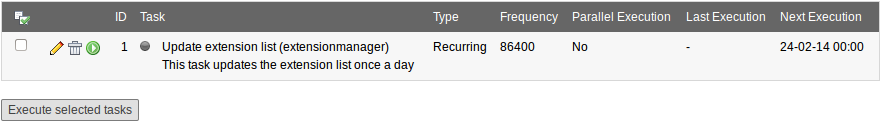
\includegraphics[width=0.95\linewidth]{Images/BackendChanges/SchedulerTaskDescriptionAsSubheader.png}
	\end{figure}

	\begin{itemize}
		\item Taskbeschreibung als Tooltip ("Hover")
	\end{itemize}

	\begin{figure}
		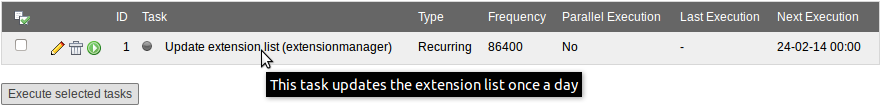
\includegraphics[width=0.95\linewidth]{Images/BackendChanges/SchedulerTaskDescriptionAsTooltip.png}
	\end{figure}

\end{frame}

% ------------------------------------------------------------------------------
% Scheduler
% ------------------------------------------------------------------------------

\begin{frame}[fragile]
	\frametitle{Änderungen im Backend}
	\framesubtitle{Planer ("Scheduler")}

	\begin{itemize}
		\item Scheduler-Tasks können nun gruppiert werden
		\item Dazu legt man auf der Root-Page (UID: 0) "Scheduler task groups" an und wählt im Task die entsprechende Gruppe aus
	\end{itemize}

	\begin{figure}
		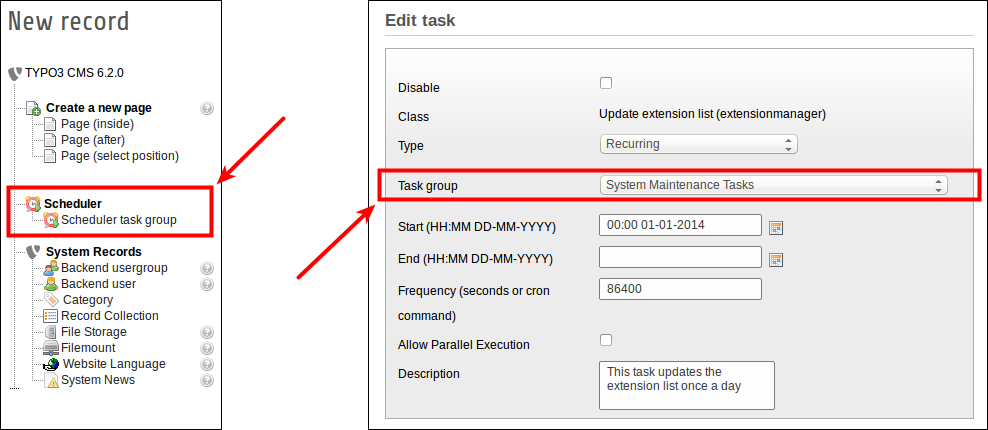
\includegraphics[width=0.85\linewidth]{Images/BackendChanges/SchedulerTaskGroup.png}
	\end{figure}

\end{frame}

% ------------------------------------------------------------------------------
% System Extension: Form
% ------------------------------------------------------------------------------
% http://forge.typo3.org/issues/38094

\begin{frame}[fragile]
	\frametitle{Änderungen im Backend}
	\framesubtitle{Systemextension: Form}

	\begin{columns}[T]

		\begin{column}{.5\textwidth}
			\begin{itemize}
				\item Neuer Post-Prozessor für das cObject FORM: \textbf{redirect}\newline
					(Weiterleitung nach Abschicken der Mail)
				\item Das Feld wird über die TypoScript-Funktion \texttt{typolink} ausgewertet,\newline
					das bedeutet, man kann z.B. eine ID für eine interne Seite oder eine URL angeben
			\end{itemize}
		\end{column}

		\begin{column}{.5\textwidth}
			\begin{figure}\vspace*{-0.4cm}
				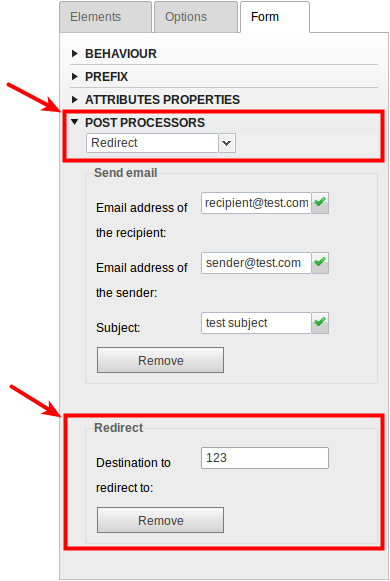
\includegraphics[width=0.65\linewidth]{Images/BackendChanges/FormRedirectPostProcessor.png}
			\end{figure}
		\end{column}

	\end{columns}

\end{frame}

% ------------------------------------------------------------------------------
% Module: List
% ------------------------------------------------------------------------------
% http://forge.typo3.org/issues/49810

\begin{frame}[fragile]
	\frametitle{Änderungen im Backend}
	\framesubtitle{Modul: List}

	\begin{itemize}
		\item Zusätzliche Spalten "UID" und "PID" in der Listenansicht für nicht-Administratoren
	\end{itemize}

	\begin{figure}
		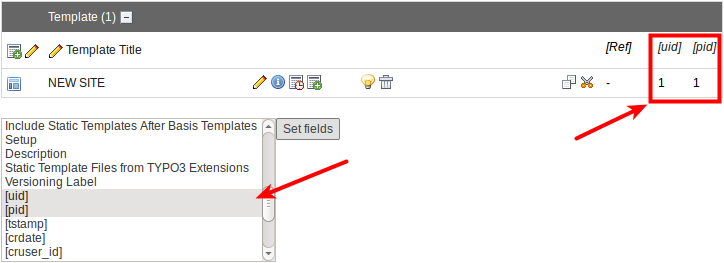
\includegraphics[width=0.95\linewidth]{Images/BackendChanges/AdditionalColumnsInListModule.png}
	\end{figure}

\end{frame}

% ------------------------------------------------------------------------------
% File Abstraction Layer
% ------------------------------------------------------------------------------
% http://forge.typo3.org/issues/50827
% http://forge.typo3.org/issues/51097

\begin{frame}[fragile]
	\frametitle{Änderungen im Backend}
	\framesubtitle{File Abstraction Layer}

	\begin{itemize}
		\item Bemerkt der FAL-Indexer eine nicht mehr vorhandene Datei, wird ein entsprechender Hinweis ausgeben und ein Flag "missing" in der Datenbanktabelle "sys\_file" gesetzt
		\item Im "Reports" Modul wird jenes ebenfalls als Warnung angezeigt
		\item Sobald die Datei wieder gefunden wird, werden Hinweis und Flag zurückgesetzt
	\end{itemize}

	\begin{columns}[T]

		\begin{column}{.5\textwidth}
			\begin{figure}\vspace*{-0.4cm}
				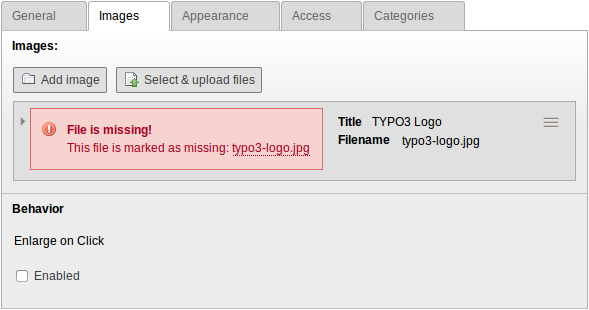
\includegraphics[width=0.9\linewidth]{Images/BackendChanges/FalMissingFileContentElement.png}
			\end{figure}
		\end{column}

		\begin{column}{.5\textwidth}
			\begin{figure}\vspace*{-0.4cm}
				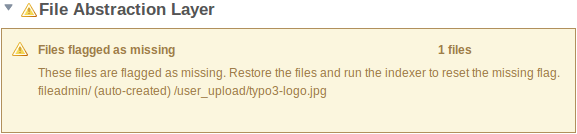
\includegraphics[width=0.9\linewidth]{Images/BackendChanges/FalMissingFileReportsModule.png}
			\end{figure}
		\end{column}

	\end{columns}

\end{frame}

% ------------------------------------------------------------------------------
% Menu/Sitemap: Categories-based Menus
% ------------------------------------------------------------------------------
% http://forge.typo3.org/issues/51161

\begin{frame}[fragile]
	\frametitle{Änderungen im Backend}
	\framesubtitle{Neuer Menütyp: Kategorien (1)}

	\begin{itemize}
		\item Im Inhaltselement "Menü und Sitemap" kann ein Menü, basierend auf Kategorien ausgewählt werden
	\end{itemize}

	\begin{figure}
		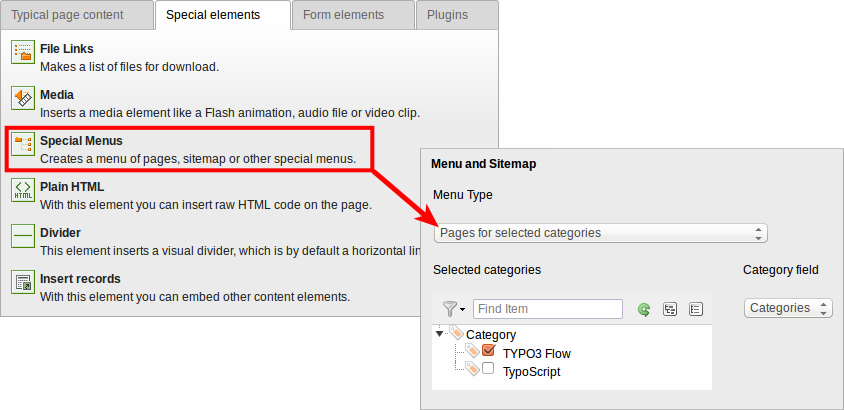
\includegraphics[width=0.8\linewidth]{Images/BackendChanges/CategoryBasedMenus.png}
	\end{figure}

\end{frame}

% ------------------------------------------------------------------------------
% Menu/Sitemap: Category-based Menus
% ------------------------------------------------------------------------------

\begin{frame}[fragile]
	\frametitle{Änderungen im Backend}
	\framesubtitle{Neuer Menütyp: Kategorien (1)}

	\begin{itemize}
		\item Weiterer neuer Menütyp: "\underline{Content elements} for selected categories"
	\end{itemize}

	\begin{figure}
		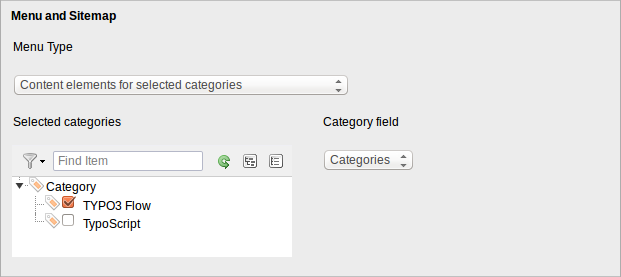
\includegraphics[width=0.6\linewidth]{Images/BackendChanges/ContentElementsForSelectedCategories.png}
	\end{figure}

\end{frame}

% ------------------------------------------------------------------------------
% Sorting Categories
% ------------------------------------------------------------------------------
% http://forge.typo3.org/issues/51590

\begin{frame}[fragile]
	\frametitle{Änderungen im Backend}
	\framesubtitle{Kategorien}

 	\begin{itemize}
		\item Kategorien können nun manuell sortiert werden\newline
			\small(bisher waren diese immer alphabetisch sortiert)\normalsize
	\end{itemize}

	\begin{figure}
		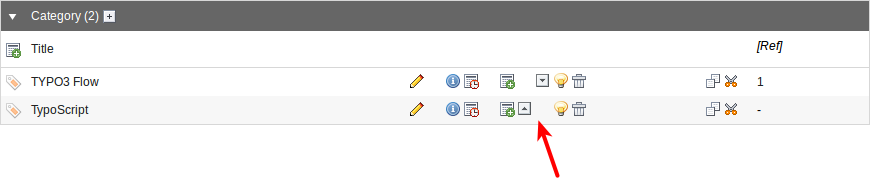
\includegraphics[width=0.95\linewidth]{Images/BackendChanges/CategorySorting.png}
	\end{figure}

\end{frame}

% ------------------------------------------------------------------------------
% Category Visibility
% ------------------------------------------------------------------------------
% http://forge.typo3.org/issues/52718

\begin{frame}[fragile]
	\frametitle{Änderungen im Backend}
	\framesubtitle{Kategorien}

 	\begin{itemize}
		\item Bei Backend-Benutzern und -Gruppen kann nun definiert werden, welche Kategorien diese sehen können
	\end{itemize}

	\begin{figure}
		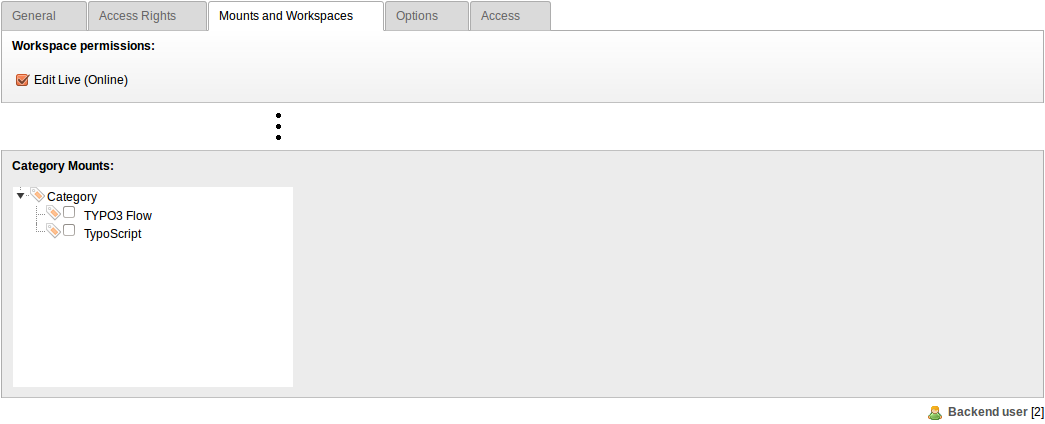
\includegraphics[width=0.95\linewidth]{Images/BackendChanges/CategoryVisibility.png}
	\end{figure}

\end{frame}

% ------------------------------------------------------------------------------
% "New Content" icon always visible
% ------------------------------------------------------------------------------
% http://forge.typo3.org/issues/48938
% http://forge.typo3.org/issues/51480

\begin{frame}[fragile]
	\frametitle{Änderungen im Backend}
	\framesubtitle{Usability}

 	\begin{itemize}
		\item Das Icon "Neues Inhaltselement" ist nun immer sichtbar, sofern die Spalte noch leer ist
	\end{itemize}

	\begin{figure}
		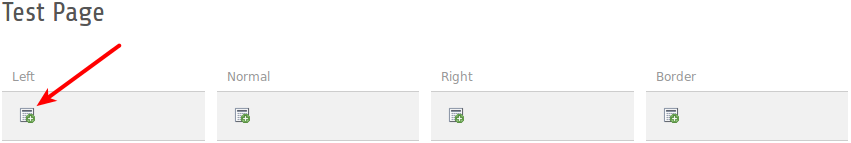
\includegraphics[width=0.95\linewidth]{Images/BackendChanges/NewContentIconAlwaysVisible.png}
	\end{figure}

\end{frame}

% ------------------------------------------------------------------------------
% Module "Functions": Hide In Menus
% ------------------------------------------------------------------------------
% http://forge.typo3.org/issues/51017

\begin{frame}[fragile]
	\frametitle{Änderungen im Backend}
	\framesubtitle{Funktionen}

 	\begin{itemize}
			\item Wenn im Modul "Funktionen" mehrere Seiten angelegt werden, kann ausgewählt werden, dass diese vorerst nicht im Menü sichtbar sein sollen
	\end{itemize}

	\begin{figure}
		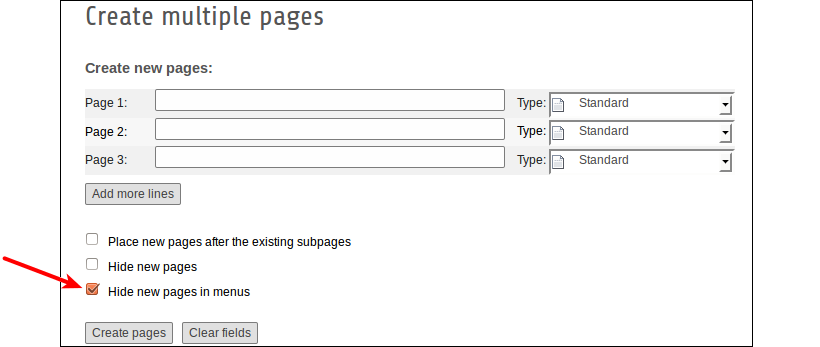
\includegraphics[width=0.85\linewidth]{Images/BackendChanges/CreateMultiplePagesHideInMenu.png}
	\end{figure}

\end{frame}

% ------------------------------------------------------------------------------
% Extension Manager: Upload Extensions
% ------------------------------------------------------------------------------
% http://forge.typo3.org/issues/51776
% http://forge.typo3.org/issues/51437

\begin{frame}[fragile]
	\frametitle{Änderungen im Backend}
	\framesubtitle{Erweiterungsmanager}

 	\begin{itemize}
		\item Extensions können nun auch im Untermenü "Erweiterungen hinzufügen" hochgeladen werden
	\end{itemize}

	\begin{figure}
		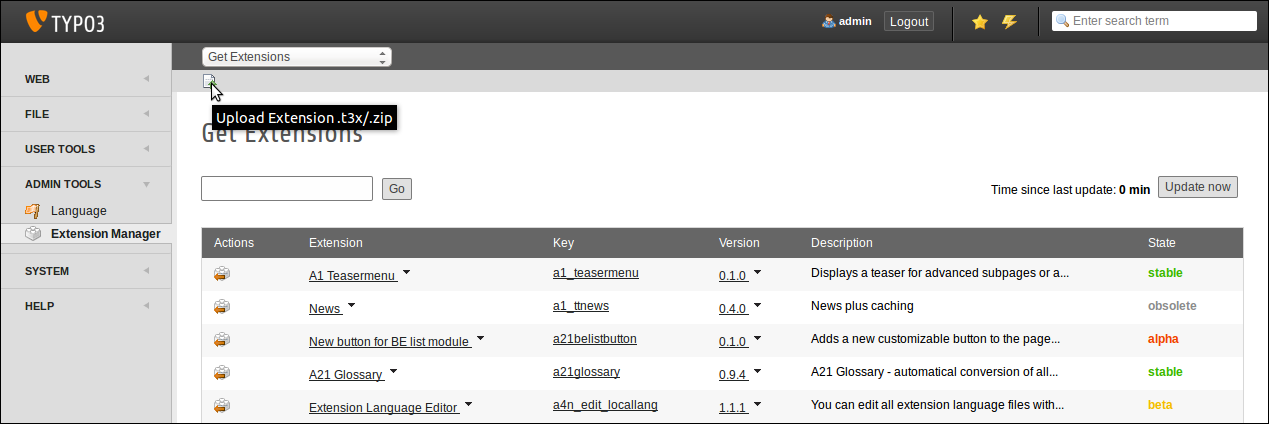
\includegraphics[width=0.95\linewidth]{Images/BackendChanges/UploadExtension.png}
	\end{figure}

\end{frame}

% ------------------------------------------------------------------------------
% Recycler
% ------------------------------------------------------------------------------
% http://forge.typo3.org/issues/52324

\begin{frame}[fragile]
	\frametitle{Änderungen im Backend}
	\framesubtitle{Recycler}

 	\begin{itemize}
		\item Einträge im Recycler lassen sich nun nach dem letzten Zugriff sortieren, um das Auffinden von Einträgen zu erleichern
	\end{itemize}

	\begin{figure}
		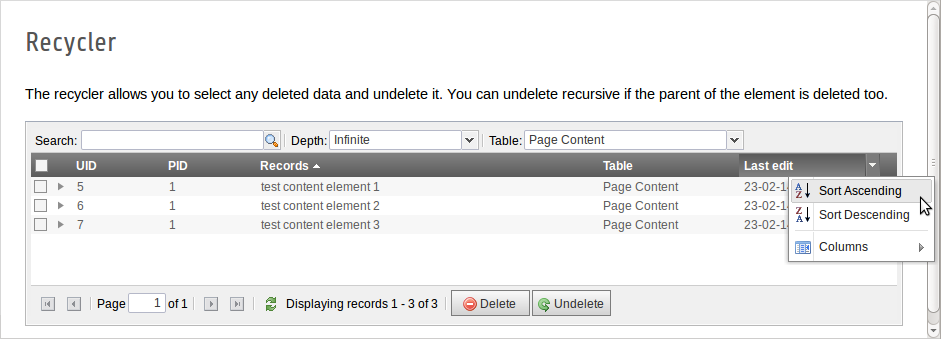
\includegraphics[width=0.95\linewidth]{Images/BackendChanges/RecyclerSortRecord.png}
	\end{figure}

\end{frame}

% ------------------------------------------------------------------------------
% File/Directory Permissions
% ------------------------------------------------------------------------------

\begin{frame}[fragile]
	\frametitle{Änderungen im Backend}
	\framesubtitle{Zugriffsreche auf Dateien und Ordner}

 	\begin{itemize}
		\item Rechte auf Dateien/Ordner können nun für Benutzer/Gruppen sehr detailiert konfiguriert werden
			\begingroup\color{typo3red}\textbf{(1)}\endgroup
		\item Jenes ist zwar bereits seit TYPO3 6.0 möglich, bisher allerdings nur mittels UserTSconfig
			\begingroup\color{typo3red}\textbf{(2)}\endgroup
	\end{itemize}

	\begin{figure}
		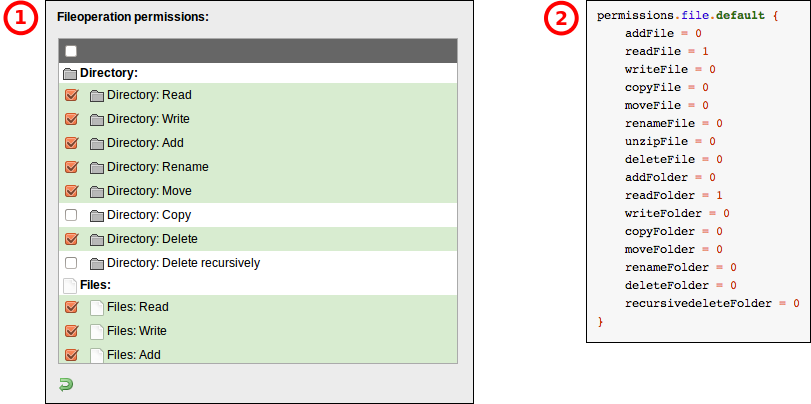
\includegraphics[width=0.65\linewidth]{Images/BackendChanges/FileAndDirectoryPermissions.png}
	\end{figure}

\end{frame}

% ------------------------------------------------------------------------------
% OpenID
% ------------------------------------------------------------------------------

\begin{frame}[fragile]
	\frametitle{Änderungen im Backend}
	\framesubtitle{OpenID (1)}

 	\begin{itemize}
		\item Die OpenID Konfiguration für Backend-Benutzer ist nun über einen Wizard wesentlich einfacher zu bewerkstelligen
		\item Hierfür ist natürlich die Systemextension EXT:openid erforderlich
	\end{itemize}

	\begin{figure}
		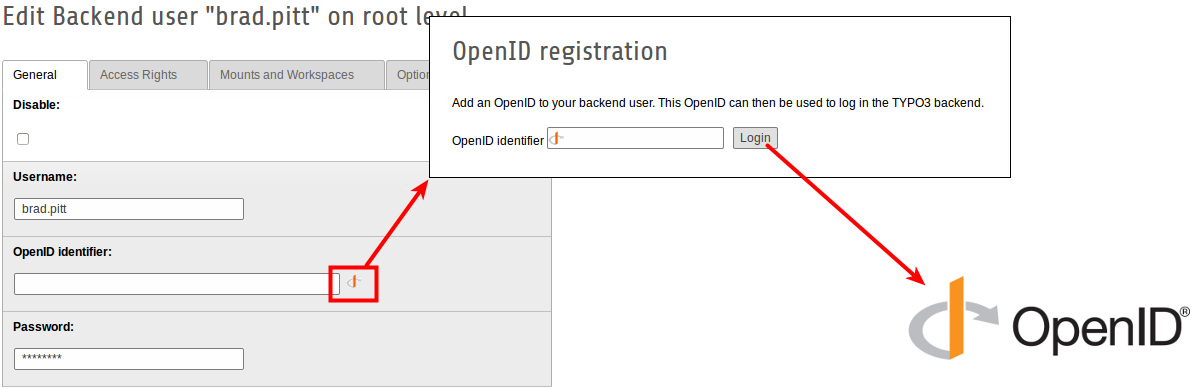
\includegraphics[width=0.95\linewidth]{Images/BackendChanges/OpenIdWizard.png}
	\end{figure}

\end{frame}

% ------------------------------------------------------------------------------
% OpenID
% ------------------------------------------------------------------------------

\begin{frame}[fragile]
	\frametitle{Änderungen im Backend}
	\framesubtitle{OpenID (2)}

 	\begin{itemize}
		\item Die OpenID Konfiguration für Backend-Benutzer ist nun über einen Wizard wesentlich einfacher zu bewerkstelligen
		\item Hierfür ist natürlich die Systemextension EXT:openid erforderlich
	\end{itemize}

	\begin{figure}
		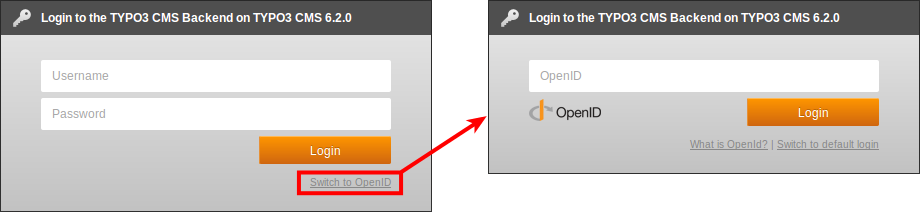
\includegraphics[width=0.8\linewidth]{Images/BackendChanges/OpenIdLogin.png}
	\end{figure}

 	\begin{itemize}
		\item Weitere Informationen über OpenID:\newline
			\small\url{http://openid.net}\normalsize
	\end{itemize}

\end{frame}

% ------------------------------------------------------------------------------
% Workspaces
% ------------------------------------------------------------------------------
% http://forge.typo3.org/issues/50223
% http://forge.typo3.org/issues/50224

\begin{frame}[fragile]
	\frametitle{Änderungen im Backend}
	\framesubtitle{Arbeitsumgebung}

 	\begin{itemize}
 		\item Benutzer können nun selbst entscheiden, an wen die Benachrichtigungen gesendet werden sollen
		\item Der Reiter "All" ist nun für \underline{alle} Benutzer (nicht nur für Admins) sichtbar
	\end{itemize}

	\begin{figure}
		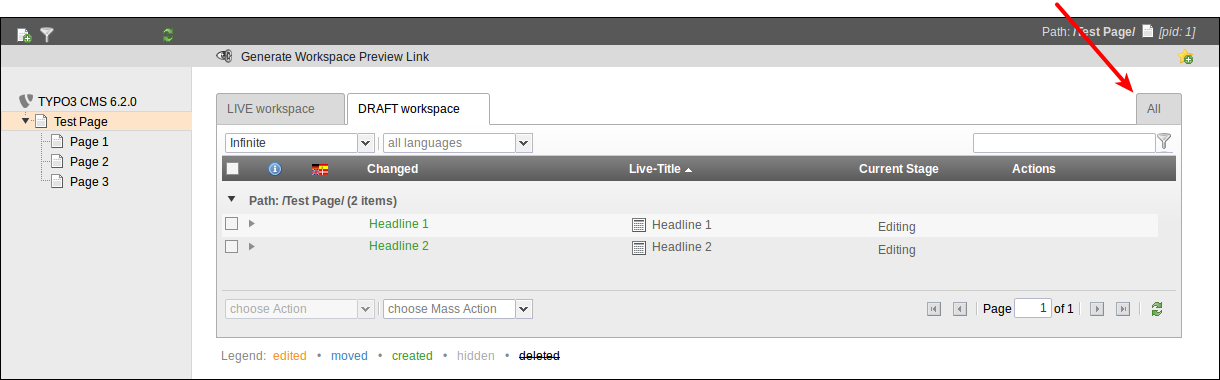
\includegraphics[width=0.95\linewidth]{Images/BackendChanges/WorkspacesTabAll.png}
	\end{figure}

\end{frame}

% ------------------------------------------------------------------------------

